\documentclass{standalone}

\usepackage{tikz}
\usetikzlibrary{calc}

\begin{document}

\begin{tabular}{c}
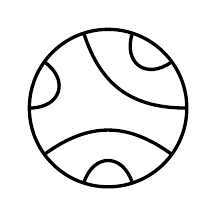
\begin{tikzpicture}[very thick]
    \draw (0, 0) circle (1);
    \draw ({360/10}:1) .. controls ({1*360/10}:.6) and ({2*360/10}:.6) .. ({2*360/10}:1);
    \draw ({0*360/10}:1) .. controls ({0*360/10}:.3) and ({3*360/10}:.3) .. ({3*360/10}:1);
    \draw ({4*360/10}:1) .. controls ({4*360/10}:.6) and ({5*360/10}:.6) .. ({5*360/10}:1);
    \draw ({7*360/10}:1) .. controls ({7*360/10}:.6) and ({8*360/10}:.6) .. ({8*360/10}:1);
    \draw ({6*360/10}:1) .. controls ({6*360/10}:.3) and ({9*360/10}:.3) .. ({9*360/10}:1);
\end{tikzpicture}
\\
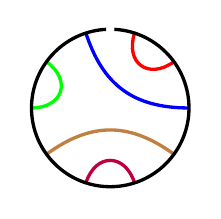
\begin{tikzpicture}[very thick]
    \draw[red] ({360/10}:1) .. controls ({1*360/10}:.6) and ({2*360/10}:.6) .. ({2*360/10}:1);
    \draw[blue] ({0*360/10}:1) .. controls ({0*360/10}:.3) and ({3*360/10}:.3) .. ({3*360/10}:1);
    \draw[green] ({4*360/10}:1) .. controls ({4*360/10}:.6) and ({5*360/10}:.6) .. ({5*360/10}:1);
    \draw[purple] ({7*360/10}:1) .. controls ({7*360/10}:.6) and ({8*360/10}:.6) .. ({8*360/10}:1);
    \draw[brown] ({6*360/10}:1) .. controls ({6*360/10}:.3) and ({9*360/10}:.3) .. ({9*360/10}:1);
    \draw (93:1) arc[start angle=93, delta angle={354}, radius=1];
\end{tikzpicture}
\\
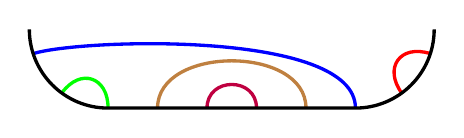
\begin{tikzpicture}[very thick]
    \draw[purple] (-{pi/10},-1) .. controls +(0,.4) and +(0, .4) .. ({pi/10},-1);
    \draw[brown] (-{3*pi/10},-1) .. controls +(0,.8) and +(0, .8) .. ({3*pi/10},-1);
    \draw[green] ($({-90-360/10}:1) + ({-pi/2}, 0)$) .. controls +({-90-360/10}:-.4) and +(0, .4) .. ({-pi/2}, -1);
    \draw[red] ($({-90+360/10}:1) + ({pi/2}, 0)$) .. controls +({-90+360/10}:-.4) and +({-90+2*360/10}:-.4) .. ($({-90+2*360/10}:1) + ({pi/2}, 0)$);
    \draw[blue] ($({-90-2*360/10}:1) + ({-pi/2}, 0)$) .. controls +({-90-2*360/10}:-.6) and +(0, 1) .. ({pi/2}, -1);
    \draw ({-1-pi/2}, 0) arc[start angle=180, delta angle=90, radius=1] -- ++({pi}, 0) arc[start angle=-90, delta angle=90, radius=1];
\end{tikzpicture}
\\
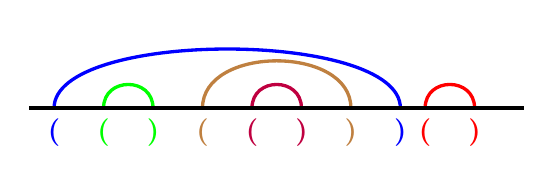
\begin{tikzpicture}[very thick]
    \draw[purple] (-{pi/10},-1) node[below]{\textbf{(}}.. controls +(0,.4) and +(0, .4) .. ({pi/10},-1) node[below]{\textbf{)}};
    \draw[brown] (-{3*pi/10},-1) node[below]{\textbf{(}} .. controls +(0,.8) and +(0, .8) .. ({3*pi/10},-1) node[below]{\textbf{)}};
    \draw[green] ({-0.7*pi}, -1) node[below]{\textbf{(}} .. controls +(0, .4) and +(0, .4) .. ({-pi/2}, -1) node[below]{\textbf{)}};
    \draw[red] ({.6*pi}, -1) node[below]{\textbf{(}} .. controls +(0, .4) and +(0, .4) .. ({.8*pi}, -1) node[below]{\textbf{)}};
    \draw[blue] ({-.9*pi}, -1) node[below]{\textbf{(}} .. controls +(0, 1) and +(0, 1) .. ({pi/2}, -1) node[below]{\textbf{)}};
    \draw ({-pi}, -1) -- ({pi}, -1);
\end{tikzpicture}
\end{tabular}

\end{document}
